\chapter{Introduction}


\section{Brief Context for the Problem}

The Domain Name System (DNS), as seen in Figure \ref{fig:dnsIntro}, translates domain names into IP addresses. This will definitely affect the daily digital interaction of each user, along with the smooth running of the Internet. Unfortunately, this one is not resistant to abuse. Meanwhile, malicious actors use DNS domains for a variety of abusive and sometimes illegal activities, such as sending malware, phishing websites, and controlling botnets \cite{so2022}. Therefore, such activity undermines the reliability and security of the Internet, posing very serious risks to cybersecurity and user trust \cite{bayer2022}. Addressing this issue requires a robust response from DNS infrastructure providers, including registrars and registries, who play a role in the management of abuse complaints. Registries refer to organisations that function to manage the top-level domains (TLDs) of the Internet, such as ".com" and ".net". On their part, registrars play a role as some form of intermediaries in the sale of domain names to the members of the public. Entities of this kind have the power to disable or deny the registration of DNS names that have been found to be abusive. But it will also consider proactive measures, such as turning down registrations that may facilitate "typosquatting", and potentially regulating permissible domain names to censor registration or renewal based on content. This would enhance the efficiency of such interventions since they shall have been transparent on the measures and the justification thereof. Although the trend is in a manner that issuing transparency reports would be able to shed light on the practices, this happens on rare occasions.

\begin{figure}[H]
    \centering
    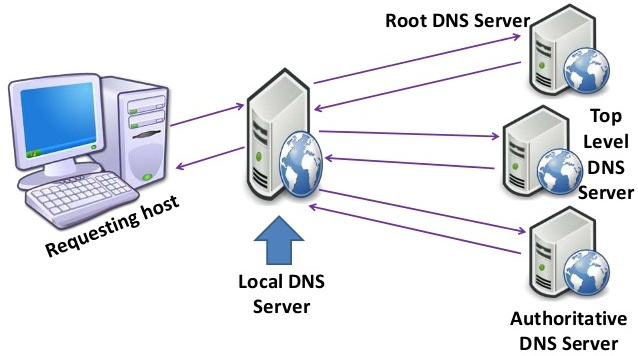
\includegraphics[width=0.4\linewidth]{introduction/dnsWork.jpg}
    \caption{How DNS works. Adapted from \cite{blanche2018understandingDNS}. }
    \label{fig:dnsIntro}
\end{figure}

\section{Motivation}

With the growing opportunities for DNS abuse for malicious and sometimes even illegal activities such as confusable domains and phishing, the figure \ref{fig:dnsintro2} of honesty and protection is at issue. This has been particularly highlighted by the harshness and regularity with which this occurs in recent studies: such as the "Study on Domain Name System (DNS) Abuse: Technical Report” by Bayer et al., which represents the need for more surveillance and moderation activities \cite{bayer2022}. Many instances of DNS abuse have not only jeopardised user protection but also shattered public trust in the digital market. As citizens become more aware of these hazards, their confidence declines, and there is a pressing need to mitigate the challenges to restore trust and a secure online environment. Hesselman et al. \cite{hesselman2020}, proposed the development of a "responsible Internet" by improving community-level transparency, as well as the responsibility to increase confidence and control. Mathew and Cheshire's analysis and self-reporting Trust and Community Practice in the Context of Network Security explore the importance of trusting interactions and communities online and depict how the danger of DNS abuse undermines it \cite{mathew2016}.

\begin{figure}[H]
    \centering
    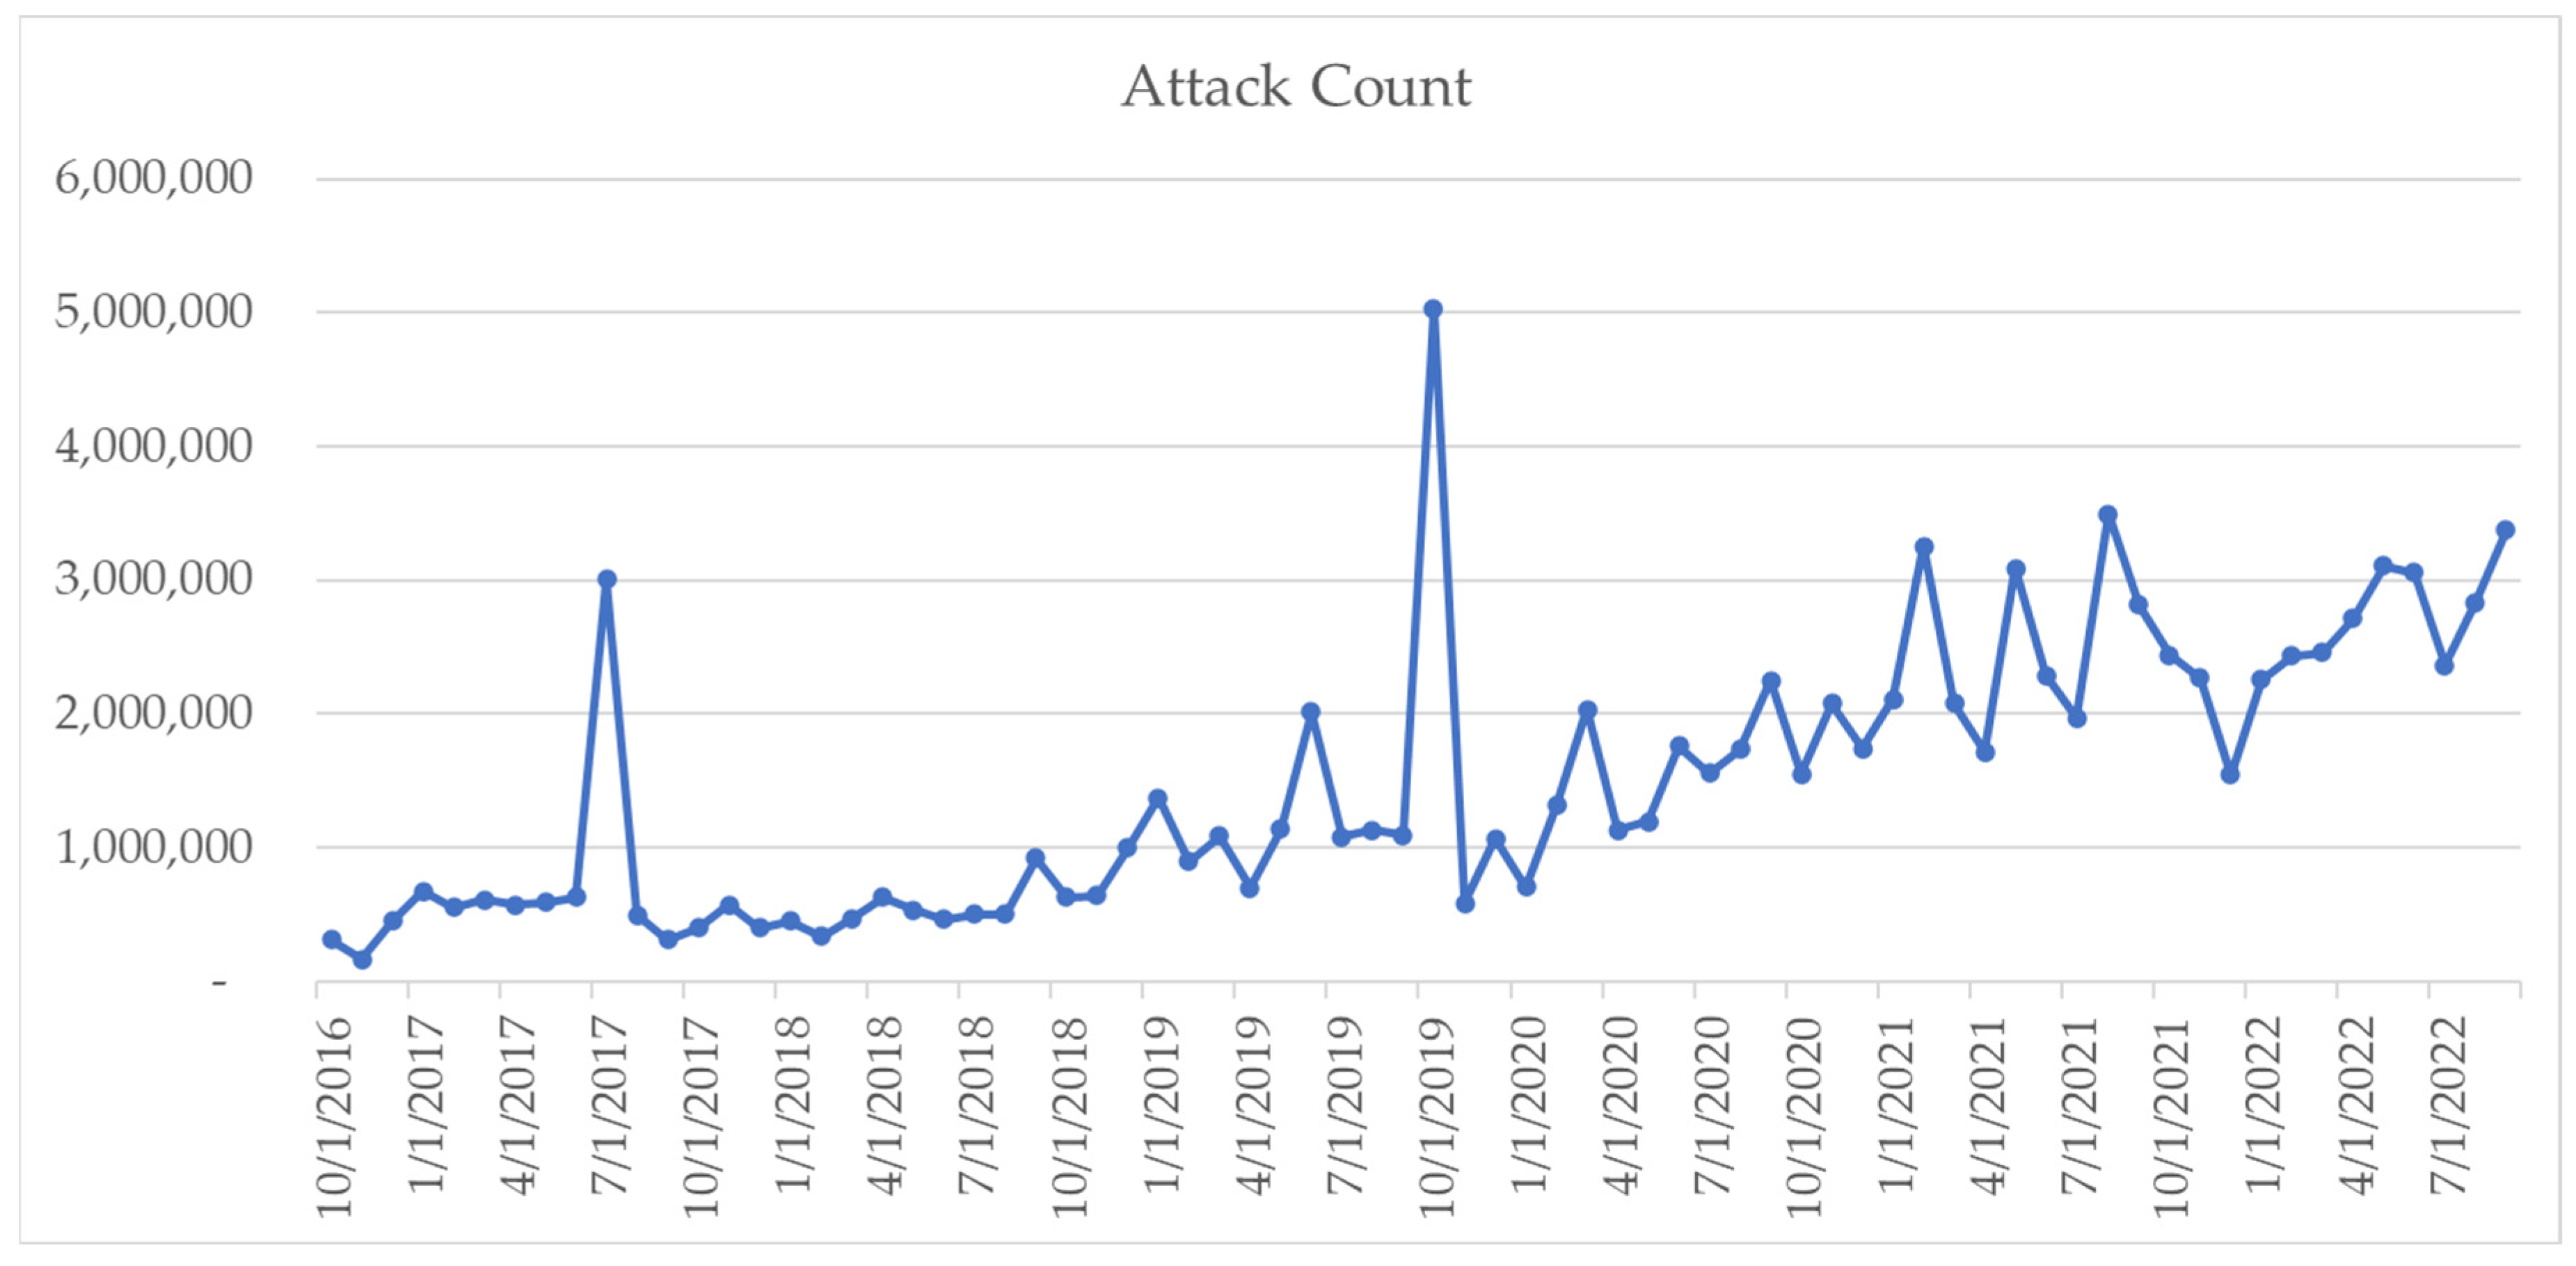
\includegraphics[width=0.5\linewidth]{introduction/maliciousActivity.png}
    \caption{ increase in DNS abuse incidents over time. Adapted from \cite{Rich2023Cyberpsychology}.}
    \label{fig:dnsintro2}
\end{figure}

Registries and registrars are leading the way in this issue, especially DNS infrastructure providers such as registrars and registries. However, their policies are probably clear and transparent to themselves, just not to outsiders.  This clear approach to handling DNS abuse allegations and their accompanying actions worsens the ongoing lack of confidence. Identified in this case are the credibility and a necessary need to protect the Internet \cite{cerf2022}. It also covers the moral and legal implications, in addition to technical aspects of DNS abuse and how one can mitigate it. This is the void to which the project is motivated to fill by exploring ways to increase the transparency of mitigation of DNS abuse. To understand current efforts, the research also sought to find the difficulties in the way of more transparent practices through an evaluation of the current landscape on transparency reports and practices among DNS infrastructure providers. The ultimate goal is to contribute to a system that can facilitate, promote, and enable better and more efficient approachable transparency in the mitigation of DNS abuse.


\section{Research Question/Project \& Personal objective} 
\subsection{Research Question}

Primary research question: "How does the work of registries, registrars, and other DNS infrastructure participants, as it appears in transparency reports, help mitigate DNS abuse, and what can be learnt from it, in terms of best practices for transparency when it comes to handling complaints related to DNS abuse?" This question seeks to uncover the mechanisms, policies, and practices in place to mitigate DNS abuse and to what extent these efforts are transparent to the public and stakeholders.

\subsection{Project Objectives}

Assess handling of abuse complaints

\begin{itemize}
  \item Examine the protocols and measures that DNS infrastructure providers use to respond to abuse complaints.
  \item Report the most common types of DNS abuse complaint received and the mechanisms applied in most cases.
\end{itemize}

Assess Transparency Levels:

\begin{itemize}
  \item Evaluate the level of transparency available in the actions taken by carriers/infrastructure providers against DNS abuse.
  \item Identify what information is made public, how it is communicated, and the frequency of disclosure.
\end{itemize}

Evaluating Against Best Practices:

\begin{itemize}
  \item Measure the results against best practices in the field to establish areas of success and failure. 
  \item Identify examples of good and poor transparency or abuse mitigation measures.
\end{itemize}

Develop recommendations :

\begin{itemize}
  \item Suggest actionable recommendations to DNS infrastructure providers to improve their abuse handling and transparency.
  \item Propose that some policy changes or initiatives be implemented to normalise and enhance such practices across the industry.
  \item Contribute to work in the future on how best practices for transparency may be developed.
\end{itemize}

Contribute to stakeholder understanding: 

\begin{itemize}
  \item Give stakeholders, including consumers, policymakers, and other providers, an understanding of the handling and transparency of DNS abuse.
  \item Develop a roadmap for further research and discussion on improving DNS trust and security.
\end{itemize}

\section{Scope}	
The Scope of this project will consider the transparency measures that registrars and registries take to mitigate DNS abuse. It will look at the collection and characterisation of transparency reports that can be obtained from registries and registrars, among others that are given the same responsibilities to mitigate abuse. Furthermore, this work will review the transparency reports developed within the current year, thus forming future work on the ways through which practices for transparency could be developed. The project discusses with different actors, as summarised in figure \ref{fig:dnsintrointro}, in the DNS ecosystem to obtain their opinions and insights on what they are currently practising and the challenges they face. This will involve establishing criteria that can be used to measure the way that the same transparency can affect the perception of the Internet user, which then relates to trust and safety. The new system will not include creating new transparency tools or systems but rather will be based on scrutiny of the current procedures and recommending changes for the better. The key objective of the study is to learn more about transparency and its impacts.  

\begin{figure}[H]
    \centering
    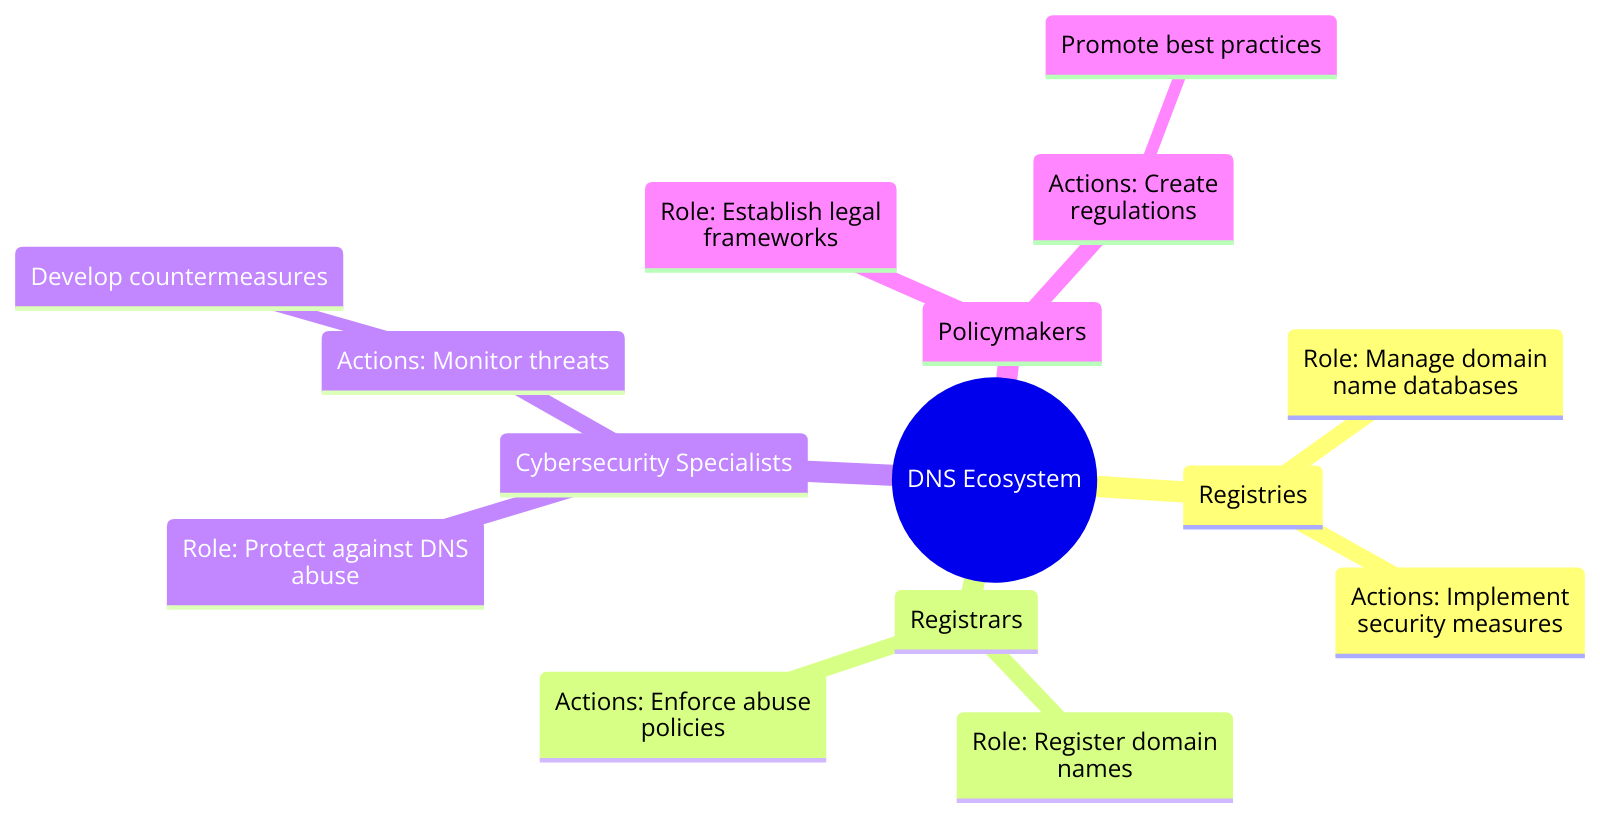
\includegraphics[width=0.7\linewidth]{introduction/diagram (8).png}
    \caption{ DNS ecosystem.}
    \label{fig:dnsintrointro}
\end{figure}

\section{ Outline of the Project Work} 

The goal of this project, "DNS Abuse Transparency", is to better understand and increase the transparency of the efforts of the registrars and registries to mitigate DNS abuse. The research will first examine the different aspects of DNS abuse, such as popular forms like phishing, confusable domains, etc. and their broader consequences. 

The questionnaire will explore the scope and effectiveness of current practices implemented on the aspect of transparency in mitigating abuse associated with the DNS. At the same time, the study will also unveil the current transparency reports that reflect the landscape, frequency, scope, and accessibility of the reports to users. Critical evaluation of the handling of DNS abuse reports forms the core of the project.

Critical evaluation of the handling of DNS abuse reports forms the core of the project. This will involve a review of proactive security controls that may be in place, procedures for mitigation, and avoidance of abusive domain registrations. Thereafter, these will be assessed in terms of how transparency influences not only user trust, but also provider reputation, and overall the effectiveness of techniques applied in mitigating abuse. The best practices for mitigating DNS abuse.

The project will discover and clarify best practices for transparency in the mitigation of DNS abuse, based on the data and insights obtained. The careful balance between security, privacy, and transparency will be taken into account by these best practices. It is under this background that the research will, therefore, with these findings in mind, develop a set of practical recommendations for the DNS infrastructure providers seeking to increase transparency for better security and, therefore, trust in the digital ecosystem.

A comprehensive timeline will guide the progress, guaranteeing an organised study of the subject. The project, upon completion, would have contributed to a collection of recommendations and considerations for further study and policy creation in this area of Internet governance. This, in turn, would give a further comprehensive understanding of where the current state of DNS abuse transparency lies.

\section{Outline of the report}

This report offers a comprehensive account of the steps performed, decisions made, and research carried out during the project's development. The format of the report is as follows:

\textbf{Chapter 2 - Background }

This chapter discusses the foundation of DNS, its importance, its weaknesses, and several types of abuse. Explaining the methods formulated in combating DNS abuse gives a specific look at the work done by ICANN and the DNS Abuse Institute.

\textbf{Chapter 3 -  State of the art }

This chapter critically looks at some of the existing strategies towards mitigation of DNS abuse and their effectiveness. This chapter will give an account of the complex relationship that international governments have with DNS and outline efforts to openness made by companies such as Google and Cloudflare. In addition to stressing the difficulties in striking a balance between user privacy and compliance requirements, the chapter emphasises the importance of DNS in internet governance. Investigate how various tactics are used and their effects on the larger online ecosystem through critical analysis.

\textbf{Chapter 4 -  Research methodology }

This chapter describes techniques to investigate DNS abuse and transparency from the infrastructure provider. The author goes on how the questionnaires were made, how the responses from stakeholders were analysed, and what kinds of DNS abuse were found. This chapter describes the methodology used to collect and examine data to understand DNS abuse reporting procedures and transparency policies.

\textbf{Chapter 5 -  Implementation }

This chapter is the practical part of the project, where all other findings are implemented, including integrating the system, the back-end, and front-end implementations, and implementation technologies that will form the system. The area that this part covers is how the DNS data are visualised with the term of abuse and how the system implementation challenges are addressed. The next section also includes the testing and validation that are performed.

\textbf{Chapter 6 -  Evaluation \& Discussion }

This chapter evaluates the way the project meets the mitigation of DNS abuse and the improvement of transparency, as well as the chapter was also used to evaluate the effectiveness of transparency in mitigating DNS abuse while evaluating security issues. Furthermore, the chapter will present the limitations of the study and the extent to which the project achieved its objectives.

\textbf{Chapter 7 -  Conclusion }

The chapter provided a summary of the project results and recommendations for improving the transparency of DNS abuse mitigation. It is important to note that no matter how difficult the situation, it is important to continue to try to improve the overall security of the DNS. As a result, there are opportunities for further research in the area discussed. More importantly, the chapter underlines the essence of collaboration and transparency in tackling DNS abuse.
